\documentclass[11pt, reqno, nocenter]{article}


\usepackage{geometry}                % See geometry.pdf to learn the layout options. There are lots.
\geometry{letterpaper}                   % ... or a4paper or a5paper or ... 
%\geometry{landscape}                % Activate for for rotated page geometry
%\usepackage[parfill]{parskip}    % Activate to begin paragraphs with an empty line rather than an indent
\usepackage{graphicx}
\usepackage{amssymb}
\usepackage{epstopdf}
\usepackage{amsmath}
\newcommand{\R}{\mathbb{R}}
\newcommand{\Rho}{\mathrm{P}}
\usepackage{hyperref}
\usepackage{parskip}
\usepackage{spverbatim}
\usepackage{dirtree}
\usepackage{bm}
\usepackage{siunitx}
\usepackage[nottoc,numbib]{tocbibind}
\usepackage{todonotes}

\DeclareGraphicsRule{.tif}{png}{.png}{`convert #1 `dirname #1`/`basename #1 .tif`.png}
\DeclareSIUnit\year{yr}


\title{Fenics Ice Sheet Model User Guide}
%\date{}                                           % Activate to display a given date or no date

\begin{document}

\maketitle

This document briefly outlines how to get started with the Fenics ice sheet model. 

\tableofcontents 


\section{Introduction}


Ice sheet models are important tools for not only generating knowledge, but also for operational forecasts. In this way, they are analagous to weather models and oceanographic models. Ice sheets currently contribute significantly to sea level rise, and this contribution is expected to increase over the coming century. With over 7 \si{\metre} of sea level rise equivalent stored in the Greenland Ice Sheet, and over 50 \si{\metre} sea level rise equivalent in the Antarctic Ice Sheet, forecasts of ice sheet evolution are crucial to informing our response to climate change.  Accurately constraining the predicted ice mass loss, as well as the uncertainty in the predictions, is important for assessing risk and implementing succesful mitigation/adaption strategies.

Most models in glaciology approach the ice sheet forecasting problem from a deterministic perspective. That is, given a set of inputs, the model will produce a single output. The evolution of this approach is to consider the problem probabilistically, calculating the probability distribution of possible answers. Knowing the posterior probability distribution allows us to consider the relative likelihood of different outcomes and establish credible intervals for outputs. Fenics Ice is an ice sheet model developed from a Bayesian statistics perspective, providing uncertainty quantification of relevant quantitites such as mass loss.

Large scale models pose unique challenges for probabilistic modelling. A key problem is the computation expense of running large scale models. Ice sheet models requiring solve a highly non-linear set of equations over large domains. Ice is commonly modelled as a viscous, creeping, incompressible fluid, shear thinning fluid, where viscosity is a function of both temperature and strain rate. Simplifications of the stokes equations based on phsyical assumptions are often used, including in Fenics Ice, for computational reasons.  Real running time of a model over a relevant domain in Antartica can be on the order of hours - days, even with specialized solvers, parallelized programming, and variable resolution. A second key problem is the extremely high dimensionality of ice sheet models. The number of parameters can range from $10^5$ - $10^9$ depending on the model approximation, domain size, and grid resolution. These problems are not unique to glaciology, and are also encountered in models such as mantle convection, weather forecasting, and ocean circulation. 

Computational expense and high dimensionality prohibit the effective use of monte carlo methods for large scale models. Two alternative approaches developed in the scientific community are Ensemble Kalman Filters and Variational Bayes. Ensemble Kalman Filters sample the posterior probability distribution using an ensemble of forecast states, estimating the forecast uncertainty based on the sampled uncertainty. The challenge is to suitably select the ensemble of model runs. Variational methods estimate the forecast uncertainty based on propogating uncertainty through the model by linearizing the model and using the adjoint. The challenge here is that that the model must be able to be automatically differentiatied.

Fenics Ice approaches uncertainty quantification of ice sheet models using the variational approach. The implementation mirrors that of \cite{Isaac2015}, who developed a framework for end-to-end uncertainty quantification of problems consisting of both data assimilation and forward run. This involves 1) inferring unobserved model parameters from data; 2) determining the uncertainty of the inferred model parameters; 3) running the forward model to make a prediction about a quantity (e.g. ice mass loss); 4) propogating the uncertainty in inferred parameters to the model prediction. The key assumptions made in this approach are that probability distributions are Gaussian, and that the forward model can be reasonably approximated by a first-order Taylor approximation.

The main glaciology problem Fenics Ice sets out to address is how the uncertainty in inverted basal drag and $\beta_{glen}$ (temperature dependent coefficient in stress-strain relationship) affect the model forecast. The aim is to understand when the uncertainty in the forecast is on the same order of magnitude as the forecast, determining a forecasting horizon. The same framework allows us to understand how uncertainty in quantities such as bed topography or ice thickness propogate through the model. Another question Fenics Ice is coded to investigate is the question of next-best-measurement. That is, given one additional measurment in a system, where would be the most informative location to place it? Fenics Ice is not limited to these questions, and can easily be adapted to address a variety of research questions. 

Fenics Ice leverages the open source FEniCS computing platform for solving partial differential equations via finite element methods \cite{AlnaesBlechta2015a}. FEniCS does not much of the computational heavy lifting, including mesh generation, implementing appropriate function spaces, and finite element assembly. Interfaces with PETSc and SLEPc provide efficient non-linear solvers and eigendecomposition algorithms. To generate the adjoint of the ice sheet model, and compute Hessian actions, Fenics Ice uses the tlm adjoint package \cite{Maddison2019}. 



\section{Installation}

The Fenics Ice model is built using the open source Python finite element software \href{https://fenicsproject.org/}{FEniCS}, and depends on the package \href{https://github.com/jrmaddison/tlm_adjoint}{tlm\_adjoint} for implementing inversion and error propagation capabilities. The script install.sh will attempt to create a suitable conda environment and install fenics\_ice. Sections below serve to document the steps of install.sh.

\subsection{Conda Environment}

fenics\_ice relies heavily on conda to manage dependencies; conda is great because it encapsulates all the dependencies in an environment which is separate from the host system, but without the overhead of running a virtual machine or docker container. The conda environment in which fenics\_ice resides is described by the top-level YAML file {\tt environment.yml}. It is called `fenics\_ice', uses the channel conda-forge, and has several package dependencies. For now Python is pinned at version 3.8 and fenics is pinned at 2019.1.0. These lines from the installation script create the fenics\_ice conda environment and activate it:

\begin{spverbatim}
conda env create -f $FENICS_ICE_BASE_DIR/environment.yml
conda activate fenics_ice
\end{spverbatim} %$

\subsection{Installation of tlm\_adjoint \& fenics\_ice}

Neither tlm\_adjoint or fenics\_ice are currently available through a conda channel or python repo. As they are both python tools, they are `installed' simply by downloading them and pointing our conda environment to their directories:

\begin{spverbatim}
#install tlm_adjoint & checkout the relevant devel branch
git clone https://github.com/jrmaddison/tlm_adjoint.git
cd $INSTALL_DIR/tlm_adjoint
git checkout jtodd/fice_devel

# Point the conda environment to tlm_adjoint & fenics_ice
conda develop $INSTALL_DIR/tlm_adjoint
conda develop $FENICS_ICE_BASE_DIR
#conda develop $INSTALL_DIR/fice_toolbox  <- Optional
\end{spverbatim}

\section{Program structure}

\subsection{Overview}

The top-level directory {\tt fenics\_ice} defines the library itself, while the {\tt runs/run\_*.py} scripts each execute a phase of a typical simulation. Section \ref{sec:uq} describes the function of each of these scripts. Several example cases are available in {\tt example\_cases}. For example, the script {\tt example\_cases/ice\_stream/run\_fwd.sh} executes every simulation phase in order, taking its configuration from the configuration file {\tt ice\_stream.toml}.

The core of the ice sheet model is in two files: {\tt /code/model.py} and {\tt /code/solver.py}. These are utilized by the python scripts in the {\tt /runs} folder, which execute specific parts of a simulation. The python scripts there are generic to any simulation. Each new simulation then has its own primary folder in the {\tt /scripts} folder, with simple bash scripts which call program files in {\tt /runs} with specific parameters and data files.

The bash scripts in {\tt /scripts} are where parameters and data file locations are specified; these are bash simple wrapper scripts for calling python scripts in {\tt /runs}. The data and parameters are used by the program files in {\tt /runs} to create a model object (via a class defined in {\tt model.py}) and subsequently a solver object (via a class defined in {\tt solver.py}). The model object contains all the necessary data for a simulation, such as topography, constants, and velocity observations for inversions. The solver object contains the ice sheet physics/inversion code. The model object is passed as a parameter to your solver object. This object then allows you to solve the SSA equations \cite{MacAyeal1989} on your domain, invert for basal drag or $B_{glen}$, and perform uncertainty quantification. The options of any python script in the {\tt /runs} folder can be viewed by typing 'python run\_xxx.py --help'.


The {\tt /aux} folder contains auxillary files; in here, the file {\tt gen\_ismipC\_domain.py} generates the ismipC domain,  based off definitions in {\tt test\_domains.py}. The {\tt /input} folder is where input files, such as topography and ice thickness, for specific simulations are located. Similarily, the {\tt /output} folder is where output is stored from specific simulations.

\subsection{Directory Structure}

The complete set of files and directories provided in the FenicsIce repository can be viewed online, using a file explorer, or with the following git command:
\begin{spverbatim}
>git ls-tree -r HEAD --name-only
\end{spverbatim}

The core structure and key files are: \\

\dirtree{%
.1 fenics\_ice.
.2 fenics\_ice.
.3 config.py.
.3 decorators.py.
.3 eigendecomposition.py.
.3 fenics\_util.py.
.3 graphviz.py.
.3 inout.py.
.3 mesh.py.
.3 minimize\_l\_bfgs.py.
.3 prior.py.
.3 optim.py.
.3 model.py.
.3 solver.py.
.3 test\_domains.py.
.2 runs.
.3 process\_eigendec.py.
.3 run\_balancemeltrates.py.
.3 run\_eigendec.py.
.3 run\_errorprop.py.
.3 run\_forward.py.
.3 run\_inv.py.
.3 run\_invsigma.py.
.3 run\_momsolve.py.
.2 example\_cases.
.3 ice\_stream.
.3 ice\_stream\_varres.
.3 ismipc\_rc\_1e6.
.3 ismipc\_rc\_1e4.
.3 ismipc\_40x40.
.3 ismipc\_30x30.
.2 tests.
.3 conftest.py.
.3 test\_runs.py.
.3 test\_model.py.
.3 test\_config.py.
.2 aux.
.3 gen\_ismipC\_domain.py.
.3 test\_domains.py.
.3 Uobs\_from\_momsolve.py.
.3 plotting.
.2 user\_guide.
.3 user\_guide.pdf.
.2 .github.
.3 workflows.
.4 test-fice.yml.
}

\subsection{Configuration files (.toml)}

{\tt fenics\_ice} uses \href{https://github.com/toml-lang/toml}{Tom's Obvious, Minimal Language} for configuration. See\\ {\tt example\_cases/ice\_stream/ice\_stream.toml} for an example.
\textbf{Tip:} emacs has a `toml-mode' package which provides syntax highlighting!

Configuration is split into sections denoted {\tt [thus]}, and the TOML file controls all aspects of a simulation, from the location of input \& output files {\tt [io]}, physical {\tt [constants]}, the definition of the {\tt [mesh]}, {\tt [ice dynamics]} and velocity {\tt [obs]}. Parameters for a specific model phase are defined in {\tt [inversion]}, {\tt [eigendec]}, {\tt [time]}, {\tt [errorprop]} and {\tt [invsigma]}.

Most parameters which can take a sensible default value do so. During development, Joe has tried to ensure that every configurable parameter appears in at least one of the example\_case .toml files. However, the best way to get \textbf{an exhaustive list of all configurable parameters and their default values} is to look at the file {\tt fenics\_ice/config.py}.

In addition to individual {\tt [sections]} describing some set of parameters, {\tt fenics\_ice} configuration files also define boundary conditions using the TOML {\tt [[list]]} specifier. Any section specifier in double brackets (e.g. {\tt [[BC]]}) can be defined multiple times, and will be parsed to a \textbf{list}. This enables us to easily specify a list of boundary conditions. More info on boundary conditions in Section \ref{sec:bc}.

The cases in {\tt example\_cases} are also used to test the model, and so they have an additional .toml section called {\tt [testing]}. More info on this in Section \ref{sec:test}

\subsection{Model \& Solver Objects}

At run time, every simulation phase begins by the definition of a {\tt model} object, usually followed by the definition of a {\tt solver} object. These classes are defined in model.py and solver.py respectively. Broadly speaking, the {\tt model} object is responsible for loading \& storing input data, initialising function spaces and functions, and setting up boundary conditions. The model object has a list member called `solvers' which, at the present stage of fenics\_ice development, will only ever point to a single {\tt solver} object, described below.

The {\tt ssa\_solver} object defined in solver.py is currently the only available solver, and it defines methods for solving both the shallow-shelf approximation (SSA), the time dependent thickness advection equation and inverse methods. It also has methods for getting the control functions from the model object, setting their values, and returning them to the model object. It also defines the Quantities of Interest, sliding laws, viscosity etc.

Overall, the current split between model/solver is overly simple and really not ideal.
Too many things are handled directly by the {\tt ssa\_solver} object which should exist as functions in other modules.
Indeed, the {\tt ssa\_solver} class should really just handle the solution of the SSA equations, and the {\tt model} object should have a separate member which handles inversions, thickness advection, the definitions of dynamics, etc.

In {\tt ssa\_solver}, {\tt def\_mom\_eq} defines the momentum equation (SSA), and {\tt def\_thickadv\_eq} defines the thickness advection equation. So these functions really represent the mathematical kernel of the model. The inverse model phase is carried out by {\tt ssa\_solver.inversion()}.

\subsection{Control Functions \& Mixed Spaces}

Work so far using {\tt fenics\_ice} has concentrated on two control functions: {\tt 
alpha} and {\tt beta}. {\tt alpha} represents the basal sliding parameter which the rest of the glaciological community calls beta... while {\tt beta} represents the rheological parameter which the rest of the community typically calls A. At this point, it's too late to turn back.

It's possible to carry out simulations where either {\tt alpha} or {\tt beta} or both are inverted for, and it's possible to eigendecompose the hessian of the cost function (J) with respect to the relevant control function(s). In the single-control case ({\tt alpha} or {\tt beta}), the control function is defined in a CG1 space ({\tt solver.Qp}). However, in the dual-control case, the control functions \textbf{must} be defined in a mixed space (CG1 x CG1, {\tt solver.QQ}) for eigendecomposition. The {\tt ssa\_solver} constructor argument {\tt mixed\_space} determines whether the control functions will form a mixed space function or separate CG1 space functions.

If you look at {\tt run\_inv.py}, you'll notice it \textbf{never} uses a mixed space.
This is because it's primarily the eigendecomposition \& subsequent operations involving the eigenfunctions which require the mixed space, and there is no tlm\_adjoint annotated connection between the inversion phase \& subsequent phases. Thus it is possible, and simplest, to simply treat the control functions as separate CG1 functions at this stage.

The logic of getting \& setting the control function values is handled by the ssa\_solver methods: {\tt get\_control, get\_control\_space, set\_control\_fns, update\_model\_fns}. Note that the {\tt model} object has members {\tt alpha} and {\tt beta}, but the solver's equivalent members are actually \textbf{copies}, so one of the last things done by the {\tt inversion} method is to copy the solver's control functions back to the model.

\subsection{Meshes} \label{sec:mesh}

FEniCS has two native mesh formats: XML (deprecated) and XDMF. Older example cases (ismipc) use the XML format, whereas newer cases (ice\_stream, Smith) use XDMF. Meshes defined in XDMF files also have a .h5 file with the same name, which stores the actual data in binary format. For example, the mesh for the ice\_stream case is in {\tt example\_cases/ice\_stream/input} and consists of the files {\tt ice\_stream.xdmf} and {\tt ice\_stream.h5}. In that directory, you'll also find an XDMF called {\tt ice\_stream\_ff.xdmf}, which defines the FEniCS `facet function' associated with the mesh. This `facet function' is used to identify boundary conditions. Section \ref{sec:bc} describes how fenics\_ice deals with BCs internally.

Meshes in fenics\_ice \textbf{must} conform to the ice domain, meaning every cell/element must be ice. Previously, meshes were defined over a whole region including ocean \& bare rock regions (nunataks), and an associated mask allowed fenics\_ice to define the ice-conforming region as a FEniCS \texttt{SubMesh}. However, {\tt SubMeshes} don't work in parallel, and other attempts to define a FEniCS {\tt Measure} on only part of a domain proved fruitless. So, we opted to abandon the attempt to use masked non-conforming meshes. Re-open that can of worms at your peril!

Figure \ref{fig:smithmesh} shows the mesh for the Smith Glacier region. Resolution is highly heterogeneous, depending on observed strain rates. The mesh was produced by the script {\tt fice\_toolbox/meshing/smith\_mesh\_metric\_mmg.py}. See Section \ref{sec:toolbox} for more info on the fice\_toolbox repo.

\begin{figure}[htbp]
  \centering
  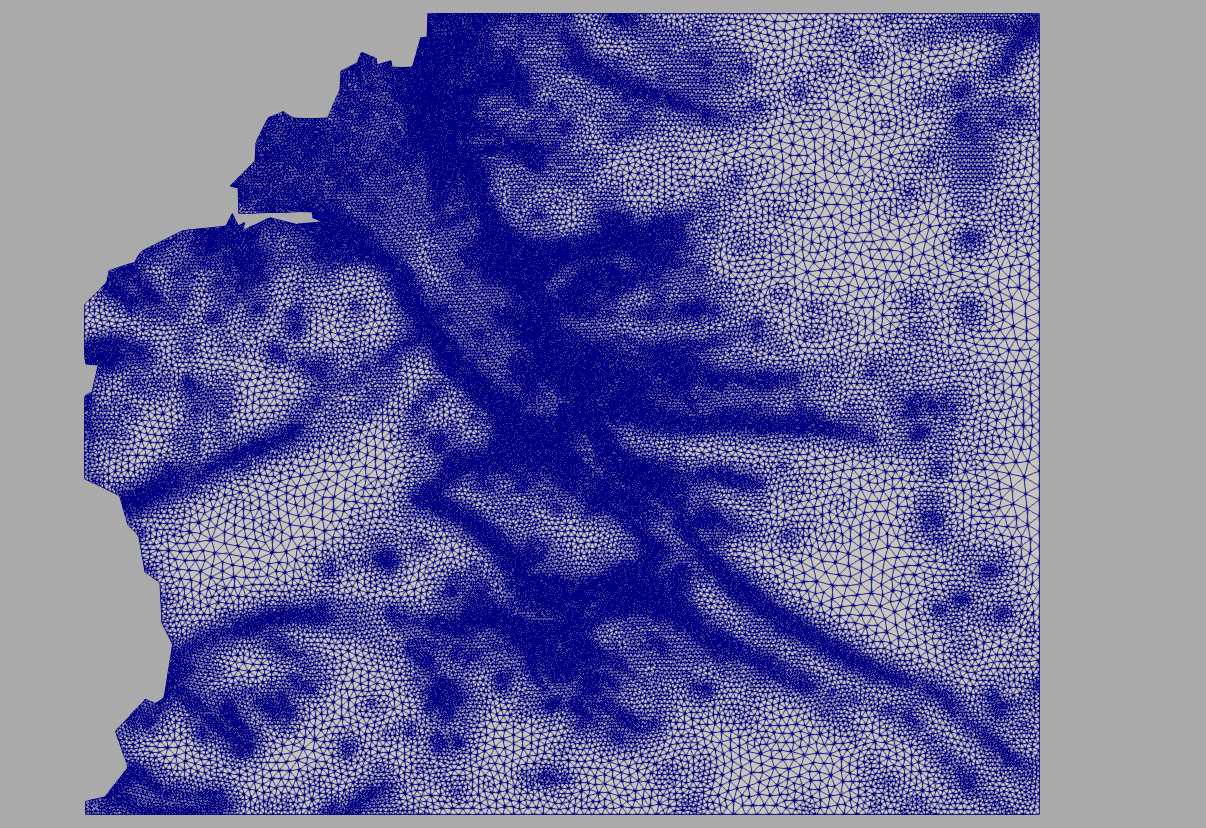
\includegraphics[width=10cm]{./figures/smith_mesh.png}
  \caption[Mesh of Smith Glacier]{Variable resolution mesh of Smith Glacier region. Mesh resolution depends on observed strain rates. The boundaries to the East and South are entirely ice-ice boundaries, whereas the North and West features calving fronts where ice meets ocean.}
      \label{fig:smithmesh}
\end{figure}


\subsection{Boundary Conditions} \label{sec:bc}

A 2D finite element mesh has 3 fundamental entity types: vertices (points), facets (edges) and cells (elements). Facets can be further divided into internal and external. For fenics\_ice boundary conditions we are exclusively concerned with \textbf{external facets}, i.e. the edges which form the domain's exterior ring. This is because we opt to work exclusively with conforming meshes, so the edge of the mesh also represents the edge of the domain.

FEniCS (actually UFL) defines 3 in-built integral `measures': {\tt dx, ds, dS}. {\tt dx} integrates over the whole domain (all cells), {\tt ds} integrates over all \textbf{external} facets, and {\tt dS} integrates over \textbf{all} facets. The latter is rarely used in fenics\_ice (only for jump conditions in DG0 forms). All boundary conditions are integrated using the in-built {\tt ds}.

Boundary conditions are defined by providing an XDMF file containing a FacetFunction. External facets are marked with integer labels, where each label value defines a single boundary. These are parsed into fenics\_ice via the {\tt model.mark\_BCs} method, which calls the function {\tt mesh.get\_ff\_from\_file}.

The name of the file containing the FacetFunction is specified in the .toml via {\tt bc\_filename} in the {\tt [mesh]} section. Each {\tt [[BC]]} section in the .toml file specifies a different boundary condition, and each BC can apply to \emph{multiple labelled boundaries}:

\begin{spverbatim}

[mesh]
mesh_filename = "ice_stream.xdmf"
bc_filename = "ice_stream_ff.xdmf"

[[BC]]
name = "Lateral Margins" # unimportant
labels = [1, 3, 4]
flow_bc = "no_slip"

[[BC]]
name = "Calving Fronts"
labels = [2]
flow_bc = "calving"

\end{spverbatim}

At present, boundary conditions for the momentum solver (SSA) are supported. Future work could conceivably add BCs for thickness advection. Boundary conditions for SSA are enforced in {\tt solver.def\_mom\_eq}. The following SSA BCs are supported:
\begin{itemize}
\item calving -- Neumann, applies the stress associated with the ice cliff force imbalance.
\item obs\_vel -- Dirichlet, applies the observed velocity.
\item no\_slip -- Dirichlet, velocity = 0.0, 0.0
\item natural -- No condition imposed
\end{itemize}

Note that the code contains references to the {\tt free\_slip} boundary condition (i.e. no penetration, no tangential friction), but this isn't actually implemented. This might be useful/essential for modelling a domain where lateral boundaries follow the direction of flow (PIG?).

\subsection{Notes on Parallelism} \label{sec:parallel}

MPI parallelism is a core feature of FEniCS, and so there's very few traces of parallel code in fenics\_ice. It's mostly implemented through the PETSc backend. For example, given a function alpha:

\begin{spverbatim}
  norm(alpha)
  norm(alpha.vector())
\end{spverbatim}

will return the function's L2 norm and the function's vector norm respectively. The same result will be returned on all processes. However, care needs to be taken when attempting to assign directly to vector values. In this case, the apply() function must be called to synchronise processes:

\begin{spverbatim}
    dg_fun.vector()[:] = nearest
    dg_fun.vector().apply("insert")
\end{spverbatim}

The code above sets the values of dg\_fun's DOFs using the numpy array {\tt nearest}.

Sometimes it's necessary to operate explicitly in parallel. See {\tt patch\_fun} in {\tt run\_invsigma.py}, which is responsible for decomposing the domain into small patches of cells over which integrals are calculated. Patch centre-points are chosen randomly, so one process (root) takes control of this operation, then broadcasts to other processes:

\begin{spverbatim}
    if root:
        if params.constants.random_seed is not None:
            random.seed(params.constants.random_seed)

        tgt_cells = random.sample(range(ncells), ntgt)
        tgt_cells.sort()
    else:
        tgt_cells = None

    # Send to other procs
    tgt_cells = comm.bcast(tgt_cells, root=0)
\end{spverbatim}

Note that non-root processes assign a value of {\tt None} to {\tt tgt\_cells}, because the symbol must be defined before being used in {\tt comm.bcast}.

It's not even necessary to partition the model mesh prior to calling the model in parallel. This is handled at run time by FEniCS. Indeed, running a model phase in parallel is as simple as:
{
\begin{spverbatim}
  mpirun -n 12 python $FENICS_ICE_BASE_DIR/runs/run_inv.py case_name.toml
\end{spverbatim}
}%$

The number of cores (e.g. 12) can simply be changed, and FEniCS will handle decomposing the mesh into the required number of partitions. It will also correctly handle outputting results in parallel too.

FEniCS has some unfortunate default behaviour with regards to OpenMP parallelism. Whereas MPI enables distributed memory parallelism (each processor addresses a different region of memory), OpenMP enables shared-memory parallelism (multi-threading). For typical fenics\_ice simulations, this actually \textbf{significantly slows down the simulation}. It is therefore recommended to ensure that the {\tt OMP\_NUM\_THREADS} environment variable is set to 1. The following section of the top-level {\tt install.sh} script ensures that the conda environment automatically sets \& unsets this environment variable:

\begin{spverbatim}
cd $CONDA_PREFIX
mkdir -p ./etc/conda/activate.d
mkdir -p ./etc/conda/deactivate.d
touch ./etc/conda/activate.d/env_vars.sh
touch ./etc/conda/deactivate.d/env_vars.sh
echo "export OMP_NUM_THREADS=1" > ./etc/conda/activate.d/env_vars.sh
echo "unset OMP_NUM_THREADS" > ./etc/conda/deactivate.d/env_vars.sh
\end{spverbatim}%$

\section{Tests \& Continuous Integration (Github Actions)} \label{sec:test}

fenics\_ice is equipped with a pytest test suite. Tests are roughly split into unit tests (\texttt{test\_config.py}, \texttt{test\_model.py}) and integration tests (\texttt{test\_runs.py}). Several test cases are provided defined on two domains: ISMIP-C and an idealised ice stream domain (ICE\_STREAM). The ISMIP-C case runs in serial only, while ICE\_STREAM is used to test the parallel capabilities of fenics\_ice. The cases in example\_cases which are used to define tests have a section at the end of their TOML config file called \texttt{[testing]}, which contains several `expected' values for various model outputs. Tests fail when the results don't match these expected values.

To run all tests for a single ISMIP-C serial case, simply:
\begin{spverbatim}
> pytest .
\end{spverbatim}
in the fenics\_ice directory. To test a specific run step (i.e. the inversion) run:

\begin{spverbatim}
> pytest -k `run_inversion'
> pytest -k `run_eigendec'
\end{spverbatim}

To run tests with iPython embed statements:
\begin{spverbatim}
> pytest -s
\end{spverbatim}

To test the parallel ICE\_STREAM case, run:
\begin{spverbatim}
> mpirun -n 2 pytest
\end{spverbatim}

\subsection{Continuous Integration with Github Actions}

Whenever a new commit is pushed to the fenics\_ice github repository, this triggers a remote test suite. This instantiates a new virtual machine, installs the just-committed version of fenics\_ice inside a conda environment, and runs both serial and parallel tests. If these tests fail, it is likely that the most recent commit has changed the behaviour of fenics\_ice in an unexpected way.

The setup for the fenics\_ice Github Actions test suite is contained entirely in the file:

\texttt{fenics\_ice/.github/workflows/test-fice.yml}

Note that the relative tolerances for the expected values are set quite high (between 1e-5 and 1e-7) because small differences in package versions between the virtual testing machine and your own machine can introduce differences. Furthermore, parallel simulations can be weakly non-deterministic, and this can be sufficient to cause tests to fail.

\subsection{Updating Tests}

Often, changes to the functionality of fenics\_ice will inevitably lead to a change in tests' expected results, and so it is necessary to update these expected values. This is easily accomplished by running the tests locally with the \texttt{--remake} flag. For example, by running both of the following commands:

\texttt{pytest --all --remake}\\
\texttt{mpirun -n 2 pytest --remake}\\

fenics\_ice will modify the `expected\_...' values for each of the TOML configuration files. These updated values can then be committed and pushed, and the tests should also pass on Github Actions.

\subsection{Taylor Verification}

The pytest test suite also incorporates Taylor verification. At present this is only implemented for the inversion and forward phases of the model.

To perform Taylor verification, use the pytest mark \texttt{tv}, e.g.:
\begin{spverbatim}
> mpirun -n 3 pytest -m `tv'
\end{spverbatim}

Pytest will then perform Taylor verification and check that the resulting \texttt{min\_order} is above 1.95. Note that the --tv option *only* runs Taylor verification, and does not test model results. At present, Taylor verification of ICE\_STREAM works better with 3 cores as opposed to 2.

Note that, for the ICE\_STREAM case, poor conditioning of the Hessian and undifferentiability of ice flotation results in failure of verification. As such, the ICE\_STREAM Taylor verification uses a value of 2 for Glen's N, and keeps the ice grounded.

\subsection{Test Failures}

If you're like me, you rely on Continuous Integration with Github Actions (GA), so you don't run the tests locally unless something goes wrong. So, in all likelihood, you've received a notification that the latest test suite has failed. My first step would be to \textbf{carefully check the log}; GA will provide you the full run logs from any run, and you can use this to discover exactly which test failed. Usually at this point, I realise that the code I've just pushed probably has an error in it. If so, see section debugging below for tips on what to do next.

Sometimes tests fail even though you haven't changed anything, or you've only changed something which couldn't \emph{possibly} have affected the test that fails (updating a README for example). In this case, my first step would be to rerun the test suite by navigating into the specific job in GA and hitting `Re-run jobs'. If it fails again, pick an earlier commit for which the tests all passed, and rerun that one. If that fails, you've got an issue with an updated external dependency. For example, the latest version of UMFPACK or BLAS, or even Python or Ubuntu has been pushed, and this is affecting your tests. To get to the bottom of this, closely compare logs from GA for runs which passed and those which failed. In one previous case, GA's default Ubuntu had been updated from 18.04 to 20.04. The solution in this case is to either pin the version that GA uses, or to update your local environment to match that of GA.

Sometimes parallel tests fail due to non-deterministic behaviour. I'm not quite sure which of fenics\_ice's dependencies cause this, but this is quite common in MPI codes. Not much to be done here except to relax your tests tolerances.

\subsection{Debugging}

If you've been modifying existing code or writing new code and you've introduced a test failure or unexpected behaviour, IPython's `embed' functionality is very useful. If you insert:

\begin{spverbatim}
from IPython import embed; embed()
\end{spverbatim}

somewhere in your code and then run the model, execution will pause at this line and drop you into an IPython shell. This allows you to poke around, check the types \& values of variables, plot things, etc. It even works for a parallel simulation, though functionality is limited because you'll only be able to control \emph{one} of the partitions.
\section{Model Output \& Paraview} \label{sec:output}

All output from a given simulation will be stored in the directory defined by \texttt{output\_dir} in the \texttt{[io]} .toml section, and all output files will be named according to the \texttt{run\_name}. This means \textbf{you can run multiple simulations in the same directory}. This makes it easy to perform a parameter sweep, so long as you remember to change the run\_name for each simulation.

A useful goal that Joe never quite got round to is to have all functions output into a \emph{single} output file. This is really useful in Paraview because it allows you to use the Calculator etc to compute combinations of variables etc. However, this doesn't seem to be supported by default in FEniCS. At least, it's certainly not possible using the old output format:

\begin{spverbatim}
outfile << function
\end{spverbatim}

If this can be implemented properly, it'd save a lot of faff with hundreds of output files for each simulation.

Don't try to compile \& install Paraview manually, it's a nightmare. Get a prebuilt binary instead. Paraview is a \textbf{really} powerful tool, but it's not very well documented. I recommend spending some time exploring the toolbars and the alphabetical list of filters.

\subsection{.pvd, .pvtu, .vtu}

A collection of files with these extensions represents a single (possibly parallel partitioned) dataset. Load the .pvd file into Paraview directly.

\subsection{.xml}

These are a (now deprecated) way to pass data from one fenics\_ice run phase to another. So, they aren't for visualisation.

\subsection{.xdmf, .h5}

These can be used for visualisation in Paraview and for passing data (e.g. Functions) between fenics\_ice run phases.

To open these for viewing in Paraview, open the .xdmf file and select either the \texttt{Xdmf3ReaderS} or \texttt{Xdmf3ReaderT}. These datasets can have multiple `timesteps' (see Paraview's top panel) which may either represent actual timesteps or, for example, the eigenvector number. As with all Paraview variables, they can also have multiple components (vectors).

For example, the eigenvector XDMF file from a dual eigendecomposition (`run\_name\_vr\_vis.xdmf') has N `timesteps', where N is the number of eigenvectors converged, and each has 3 components (alpha, beta, None). Paraview adds a 3rd dummy component to 2-component vectors.

\subsection{.p}

These are Python pickle files and, as such, can contain arbitrary data. They are typically used for data which doesn't `map' into physical space, such as the eigenvalues, the mean \& standard deviation of QoIs through time. They are opened via pickle.load in a Python script.

\section{fice\_toolbox} \label{sec:toolbox}

The repository \href{https://github.com/EdiGlacUQ/fice_toolbox}{{\tt fice\_toolbox}} contains \textbf{some pretty useful stuff} which Joe felt were worth saving but which didn't quite make sense in the fenics\_ice repository. For example, some of the files are larger than typically stored in a git repo.
So, to avoid bloat of the fenics\_ice repo, I've stored them separately. The structure is: \\

\dirtree{%
.1 fice\_toolbox.
.2 cases.
.3 ice\_stream.
.3 ice\_stream\_var\_res.
.3 ice\_stream\_wide.
.3 ismipc\_test.
.3 Smith.
.2 meshing.
.3 meshtools.py.
.3 smith\_mesh\_metric\_mmg.py.
.2 scripts.
.3 smith\_l\_curve\_rough.py.
.3 param\_sweep.py.
.2 tests.
.3 all sorts...
}

There should be READMEs all over that repository, so the following notes are to give a broad view of what you'll find there.

\subsection{cases}

This directory contains all the files/scripts needed to create all the cases that we've worked with, including ice\_stream and the Smith Glacier case. It also contains some .toml files for various simulations using those cases.

The files in the Smith case directory include scripts for processing BedMachine data into a fenics\_ice ready format, interpolating Frank Pattyn's temperature fields, etc. It also contains various notes that Joe wrote when he was developing for the Smith case.

\subsection{meshing}

The script {\tt smith\_mesh\_metric\_mmg.py}, which makes use of {\tt meshtools.py}, generates the Smith irregular mesh. This might be \textbf{very useful} for making other domains quickly. {\tt meshtools.py} is a loosely defined library with various useful functions.

\subsection{scripts} \label{sec:scripts}

Two pretty useful scripts in here.

{\tt param\_sweep.py} will take a .toml file, a parameter name, and a range, and automatically produce a series of .toml files which sweep the requested parameter. It also produces a shell script which will call {\tt run\_inv.py} for each .toml. This script \textbf{saved me a lot of time} when doing L-curves.

{\tt smith\_l\_curve\_rough.py} takes a `glob' defining a series of runs and plots the L-curve.

\subsection{tests}

This is a sort of scratch space where I've tested out loads of little fenics snippets as Proof of Concept or just to investigate behaviour. I committed it in the hopes it'll prove useful.

\section{Tutorial: A Walkthrough of IsmipC}

\textbf{This section provides a tutorial for the IsmipC simulation. However, at least some of the information here is likely to be out of date. A walk through of the Smith Glacier case is described in Section \ref{sec:smith}. This tutorial is left here in case it provides useful information not covered there.}

The Ice Sheet Model Intercomparison Project for Higher-Order ice sheet Models (ISMIP-HOM) provides a standardized set of idealized tests for ice sheet models. In this walkthrough, we apply FenicsIce to the domain prescribed by experiment C (IsmipC). A description of IsmipC is provided in Section \ref{IsmipC} of this user guide. The original IsmipC is a static simulation, meaning time evolution is not considered. We'll extend it by running a dynamic simulation for the purposes of performing uncertainty quantification.


\subsection{Generating the Domain}

Navigate to the {\tt /fenics\_ice} base directory. Activate the fenics conda environment.

\begin{verbatim}
> conda activate fenics 
\end{verbatim}

To begin, we'll generate the synthetic domain defined by the IsmipC experiment. The specifications are coded in the file {\tt /aux/test\_domains.py}. We'll use the python script {\tt gen\_ismipC\_domain.py} to create a domain with a given length and resolution.

\begin{verbatim}
> cd $FENICS_ICE_BASE_DIR/aux 
> python gen_ismipC_domain.py -o ../input/ismipC -L 40000 -nx 100 -ny 100 
\end{verbatim}

This will generate a square domain with side-length 40\si{\kilo\metre}, at a grid resolution of 100 x 100 cells, placing the output in the folder {\tt input/ismipc}.
Let's observe the files that are generated.

\begin{spverbatim}
> ls $FENICS_ICE_BASE_DIR/input/ismipC
B2.xml  Bglen.xml  alpha.xml  bed.xml  bmelt.xml  data_mask.xml  data_mesh.xml  grid_data.npz smb.xml  thick.xml 
\end{spverbatim}

The .xml files contain discretized scalar fields over the IsmipC domain on a FEniCS mesh. The extension .npz indicates a numpy file format, and contains the domain resolution and length.

\begin{itemize}
\item B2.xml -- $\beta^2$ coefficient for linear sliding law $(\bm{\tau_b} = \beta^2 \bm{u})$
\item  Bglen.xml -- parameter in Glen's flow law
\item alpha.xml -- variable in sliding law 
\item bed.xml -- basal topography
\item bmelt.xml -- basal melt. 
\item mask.xml -- mask of our domain
\item mesh.xml -- FEniCS mesh
\item smb.xml -- surface mass balance
\item thick.xml -- ice thickness

\end{itemize}

\subsection{Solving the Momentum Equations}

Having generated the files which describe our domain, we can solve the SSA momentum equations to determine ice velocities. 

\begin{spverbatim}
> cd $FENICS_ICE_BASE_DIR/scripts/ismipc/ 
> ./forward_solve.sh

Generating new mesh                                                                                                                                              
Building point search tree to accelerate distance queries.                                                                                                       
Computed bounding box tree with 39999 nodes for 20000 points.                                                                                                    
Solving nonlinear variational problem.                                                                                                                             
Newton iteration 0: r (abs) = 1.585e+03 (tol = 1.000e-08) r (rel) = 1.000e+00 (tol = 5.000e-02)                                                                 
Newton iteration 1: r (abs) = 1.139e+02 (tol = 1.000e-08) r (rel) = 7.186e-02 (tol = 5.000e-02)                                                                 
Newton iteration 2: r (abs) = 1.307e+02 (tol = 1.000e-08) r (rel) = 8.248e-02 (tol = 5.000e-02)                                                                  
Newton iteration 3: r (abs) = 9.443e+01 (tol = 1.000e-08) r (rel) = 5.958e-02 (tol = 5.000e-02)                                                                  
Newton iteration 4: r (abs) = 5.682e+01 (tol = 1.000e-08) r (rel) = 3.585e-02 (tol = 5.000e-02)                                                                 
Newton solver finished in 5 iterations and 5 linear solver iterations.                                                                                         
Solving nonlinear variational problem.                                                                                                                          
Newton iteration 0: r (abs) = 6.650e+01 (tol = 1.000e-05) r (rel) = 1.000e+00 (tol = 1.000e-05)                                                                 
Newton iteration 1: r (abs) = 4.913e+00 (tol = 1.000e-05) r (rel) = 7.387e-02 (tol = 1.000e-05)                                                                  
Newton iteration 2: r (abs) = 4.393e-02 (tol = 1.000e-05) r (rel) = 6.606e-04 (tol = 1.000e-05)                                                                 
Newton iteration 3: r (abs) = 5.647e-06 (tol = 1.000e-05) r (rel) = 8.492e-08 (tol = 1.000e-05)                                                                 
Newton solver finished in 4 iterations and 4 linear solver iterations.                                                                                           
Time for solve: 4.667648553848267      

ls $FENICS_ICE_BASE_DIR/input/ismipC/momsolve
...
\end{spverbatim}

The script automatically places the output in the subdirectory of {\tt input/}. We'll use the velocities we solved for in the next step, generating synthetic observations.

Opening {\tt forward\_solve.sh} with any text editor, we can confirm that this is a simple wrapper script.

\begin{spverbatim}
#!/bin/bash
set -e

BASE_DIR=$FENICS_ICE_BASE_DIR
RUN_DIR=$BASE_DIR/runs

INPUT_DIR=$BASE_DIR/input/ismipC
OUTPUT_DIR=$INPUT_DIR/momsolve

cd $RUN_DIR

python run_momsolve.py -b -q 0 -d $INPUT_DIR -o $OUTPUT_DIR
\end{spverbatim}

The bash script specifies key folders, that we are solving momentum equations on a domain with periodic boundary conditions (-b option), and that we are using a linear sliding law (-q 0).

\subsection{Generating Synthetic Observations}

IsmipC is a synthetic experiment, meaning we don't have observational data of ice velocities. We can generate pseudo-oberservations by adding gaussian noise to the solved velocities. We'll assume the noise is additive rather than a multiplicative factor. 

The python script {\tt Uobs\_from\_momsolve.py} takes the vector field in U.xml and generates the files: vel\_mask.xml, u\_obs.xml, v\_obs.xml, u\_std.xml, and v\_std.xml. The first file identifies where velocity data is available, the next two files contain the pseudo-observations in the x and y directions, with the final two files containing the standard deviation of the gaussian noise applied. In this case the standard deviatiation has a constant value of 1.0.

\begin{spverbatim}
> cd $FENICS_ICE_BASE_DIR/aux/
> python Uobs_from_momsolve.py -b -L 40000 \
-d $FENICS_ICE_BASE_DIR/input/ismipC/momsolve
> find $FENICS_ICE_BASE_DIR/input/ismipC/momsolve \
-type f -regex `.*\(obs\|std\).xml'
/mnt/c/Users/ckozi/Documents/Python/fenics/fenics_ice/input/ismipC/u_obs.xml
/mnt/c/Users/ckozi/Documents/Python/fenics/fenics_ice/input/ismipC/u_std.xml
/mnt/c/Users/ckozi/Documents/Python/fenics/fenics_ice/input/ismipC/v_obs.xml
/mnt/c/Users/ckozi/Documents/Python/fenics/fenics_ice/input/ismipC/v_std.xml
\end{spverbatim} %$

Copy the five files generated into {\tt \$FENICS\_ICE\_BASE\_DIR/input/ismipC/}. A study site in Antarctica or Greenland would require generating these files  from a surface velocity dataset such as NSIDC MEaSUREs.

\begin{verbatim}
> cd $FENICS_ICE_BASE_DIR/input/ismipC/momsolve
> cp mask_vel.xml u_*.xml v_*.xml ..
\end{verbatim}

\subsection{Uncertainty Quantification} \label{sec:uq}

FenicsIce is developed with an aim of understanding uncertainty in ice sheet simulations. Because inversions for key ice-sheet model variables (basal drag and $B_{glen}$) solve under-determined systems of equations, the solutions may have large, and spatially varying error distributions. The novel capabality of FenicsIce is to propogate this uncertainty through a forward stepping simulation, allowing us to calculate the probability distribution of a quantity-of-interest through time, rather than a point estimate. 

The bash scripts starting with the prefix {\tt uq\_} in {\tt scripts/ismipc} perform the uncertainty quantification process. The suffixes relate to various values of parameters. Uncertainty quantification can be seperated into five parts, corresponding to to different python scripts in the {\tt runs/} folder.

Beyond the specification of parameters and data sources, the uncertainty quantification scripts call the following (in order):

\begin{enumerate}
	\item {\tt run\_inv.py} -- Invert for basal drag
	\item {\tt run\_forward.py} -- Timestep the simulation forward in time
	\item {\tt run\_eigendec.py} -- Run the eigen-decomposition of a hessian matrix -- allowing us to multiply by the inverse of the covariance matrix of basal drag.
	\item {\tt run\_errorprop.py} -- Run the error-propogation code to calculate the uncertainty in a quantity of interest through time arising from uncertainty in the inverted values of basal drag
	\item {\tt run\_invsigma.py} -- Calculate the spatial distribution of the standard deviation of the inverted quantity.
\end{enumerate}


Steps (2) and (3) are independent of each other, and only depend on step (1). Hence their order can be switched. Step (4) depends on (1)-(3), while step (5) depends on (1) and (2).

There are five scripts pertaining to uncertainty quantification in {\tt scripts/imsipc/}.
\begin{enumerate}
	\item {\tt uq\_rc\_1e4.sh  }
	\item {\tt uq\_rc\_1e6.sh}
	\item {\tt uq\_30x30.sh  }
	\item {\tt uq\_40x40.sh  }
	\item {\tt run\_all.sh}  
\end{enumerate}

The first two bash scripts specify simulations with different levels of regularization for the inversion. Script {\tt uq\_rc\_1e4.sh} has less regularziation and results in high frequency features in basal drag. The script {\tt uq\_rc\_1e6.sh} increases the level of regularization by two orders of magnitude, so that the inverted basal drag field mirrors the specification by IsmipC. Grid resolution is the focus of the next two scripts. The scripts {\tt uq\_30x30.sh} and {\tt uq\_40x40.sh} use the regulariztion of simulation {\tt uq\_rc\_1e6.sh}, but increase the resolution to 30x30 and 40x40 respectively. The final script -- {\tt run\_all.sh}  -- simply runs the other four scripts.

We'll proceed with script {\tt uq\_rc\_1e6.sh}. To run uncertainty quantification of IsmipC, simply call the bash script:
\begin{verbatim}
> cd $FENICS_ICE_BASE_DIR/scripts/ismipc/
> ./uq_rc_1e6.sh
...
\end{verbatim}

There will be a significant amount of output. 

On a Dell XPS laptop with Intel(R) Core(TM) i7-9750H CPU @ 2.60GHz and 32GB of RAM, running Python via the Windows 10 Linux Subsystem (WSL v1.0) the script had the following timings:   

real	\hspace{10mm} 8m27.972s \\
user  \hspace{9mm}  32m10.906s \\
sys    \hspace{11mm} 21m14.797s. \\

These can be obtained in linux shell by executing {\tt time ./uq\_rc\_1e6.sh}. Let's break down the contents of the {\tt uq\_rc\_1e6.sh} script.

The script begins by defining the locations of inputs and outputs.

\begin{spverbatim}
BASE_DIR=$FENICS_ICE_BASE_DIR
RUN_DIR=$BASE_DIR/runs

INPUT_DIR=$BASE_DIR/input/ismipC
OUTPUT_DIR=$BASE_DIR/output/ismipC/ismipC_inv6_perbc_20x20_gnhep_prior
EIGENDECOMP_DIR=$OUTPUT_DIR/run_forward
FORWARD_DIR=$OUTPUT_DIR/run_forward

EIGFILE=slepceig_all.p
\end{spverbatim}

The variable {\tt OUTPUT\_DIR} should be unique to this specific simulation. The other directories are standard and do not need to be modified. The variable {\tt EIGFILE} specifies the name of the file where the output of eigendecomposition is stored. 

The current name reflects the fact that the eigenvalues and eigenvectors were calculated using the library SLEPc, and that all eigenvectors/values where calculated. Future releases plan to offer additional libraries to solve the eigenvalue problem. For large domains, calculating all eigenvectors/values is not necessary, nor feasible. 

Next in the script we define the values of parameters that will be used as command line arguments. These will be discussed in the context of the python script they're applicable to.
\begin{spverbatim}
RC1=1.0
RC2=1e-2
RC3=1e-2
RC4=1e6
RC5=1e6

T=30.0
N=120
S=5

NX=20
NY=20

QOI=1
\end{spverbatim}

The core of the script are the following lines. To see a complete list of options for each of the these python scripts, execute them with the '--help' flag (e.g. {\tt python run\_inv.py --help}).


\begin{spverbatim}
cd $RUN_DIR

python run_inv.py -b -x $NX -y $NY -m 200 -p 0  -r $RC1 $RC2 $RC3 $RC4 $RC5 -d $INPUT_DIR -o $OUTPUT_DIR
python run_forward.py -t $T -n $N -s $S -i $QOI -d $OUTPUT_DIR -o $FORWARD_DIR
python run_eigendec.py -s -m -p 0   -d $OUTPUT_DIR -o $EIGENDECOMP_DIR -f $EIGFILE
python run_errorprop.py -p 0 -d $FORWARD_DIR -e $EIGENDECOMP_DIR -l $EIGFILE -o $FORWARD_DIR
python run_invsigma.py -p 0 -d $FORWARD_DIR -e $EIGENDECOMP_DIR -k $EIGENVECTOR_FILE -l $EIGENVALUE_FILE -d $OUTPUT_DIR -o $FORWARD_DIR

\end{spverbatim}%$

The first python script {\tt run\_inv.py} performs the inversion. The {\tt -b} flag indicates that periodic boundary conditions should be applied at the domain boundary. Currently periodic boundary conditions cannot be specified on individual boundaries, but rather for the entire domain . Each of {\tt -x} and {\tt -y} specify the resolution in the number of cells in the x and y directions. At the present stage, resolution needs to be uniform in both axis. The {\tt -m} option specifies that a maximum of 200 iterations of gradient descent be performed to minimize the cost-function, while the input {-p 0} indicates we are optimizing basal drag. In the case of IsmipC, $B_{glen}$ is assigned a constant value. Scaling constants in the cost function for the inversion are specified by the {\tt -r} option. The first value scales the velocity misfit, RC2 and RC4 apply to the regularization of alpha, RC3 and RC5 apply to the regularization of beta. RC2 and RC3 specify the delta parameters in the cost function, and RC4 and RC5 specify the gamma parameters. The options {\tt -d} and {\tt -o} specify input and output directoies.

The second python script {\tt run\_forward.py} numerically integrates the simulation forward in time and calculates the adjoint of the quantity of interest with respect to the specified variable. The {\tt -t} option determines the number years to run the simulation for, with {\tt -n} number of timesteps. The $-s$ parameter specifies the numer of sensitivities to calculate. If the value is 1, than the sensitivity at the last timestep is calculated. Otherwise they are calculated at np.linspace(0, run\_length, number\_of\_sensitivites). The sensitivities of a quantity of interest are calculated. Here, we specify the quantity of interest as the integral of the height squared with the {\tt -i 1} option, as the IsmipC simulation is mass-conserving due to the periodic-boundary conditions. The other available option, suitable to real life domains, is volume above floation. Again, the options {\tt -d} and {\tt -o} specify input and output directories.

The third python script {\tt run\_eigendec.py} eigendecomposes the Hessian of the inversion cost function. The {\tt -s} flag specifies that the SLEPc library should be used, presently the only functioning option. To consider only the velocity misfit portion of the cost function, we set the {\tt -m} flag. As for {\tt run\_inv.py}, we set {\tt -p 0} to consider only basal drag. The remaining options specify the input and output locations. 

The fourth python script {\tt run\_errorprop.py} assembles the output of {\tt run\_forward.py} and {\tt run\_eigendec.py} to determine the standard deviation of the quantity of interest through time. The options for this script duplicate those above.

Lastly, the fifth python script {\tt run\_invsigma.py} processes the output of {\tt run\_eigendec.py} to determine the standard deviation of the inverted value across the domain. The options for this script duplicate those above.

\subsection{Plotting}

This section will go through plotting the results of the IsmipC experiments. It assumes you ran all the simulations in {\tt ismipc/scripts/}. If not, you'll need to execute {\tt run\_all.sh} in that folder. The timings on the same machine as previously are:

real    \hspace{10mm}79m31.631s         \\                                                                                            
user   \hspace{8mm} 350m12.844s      \\                                                                                               
sys     \hspace{11mm}215m26.250s    \\

\subsubsection{Inversion Results}
The first plot we'll create allows us to examine the inversion results. We'll do this by running the python script {\tt plot\_inv\_results.py}. You can modify the simulation and output location at the top of the script. The default simulation is {\tt uq\_rc\_1e6} and the default output location is a the folder {\tt \$FENICS\_ICE\_BASE\_DIR/output/ismipC/uq\_rc\_1e6/plots}. The script will create the a file named {\tt inv\_results.pdf} there.

\begin{spverbatim}
>cd $FENICS_ICE_BASE_DIR/output/ismipC/
>python plot_inv_results.py
\end{spverbatim} %$

There are five panels in the output plot. The inverted basal drag from the inversion is shown in panel  \textbf{(a)}, and the uncertainty in panel  \textbf{(b)}. Panels  \textbf{(c)}-\textbf{(e)} visualize how well the inversion recreates the pseudo-observed velocities. 

Figure \ref{fig:inv_results_rc1e6} displays the results with higher regularization ({\tt uq\_rc\_1e6}) while Figure \ref{fig:inv_results_rc1e4} shows the results with lower regularization. Observe that less regularization results in higher frequencies in the pattern the basal drag coefficient.

\begin{figure}[!htbp]
  \centering
  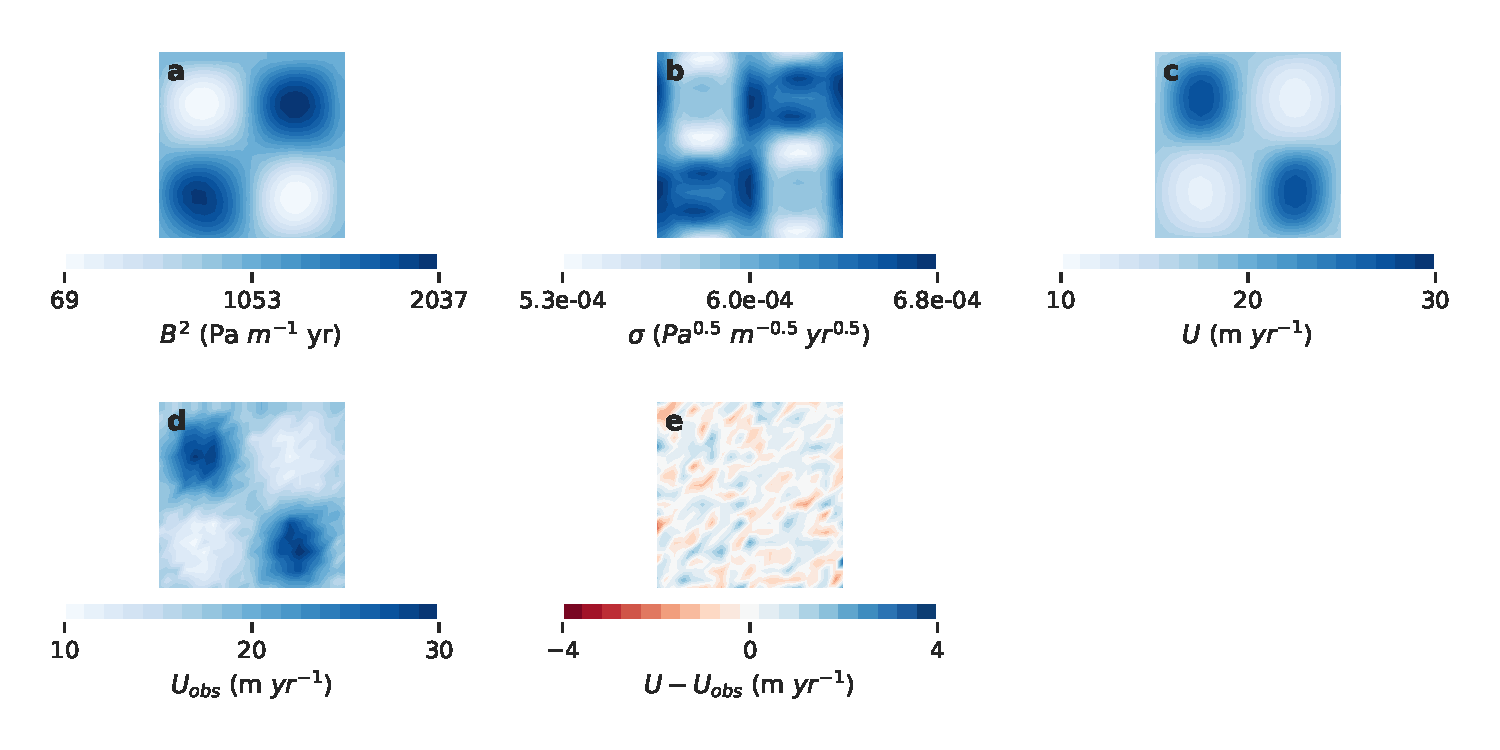
\includegraphics[width=13cm]{./figures/inv_results_rc1e6.pdf}
  \caption[IsmipC Inversion Results for High Regularization.]{IsmipC inversion results for higher regularization. \textbf{(a)} linear coefficient in basal sliding law;  \textbf{(b)} standard deviation of alpha (defined in this experiment as the square root of the linear drag coefficient);   \textbf{(c)} modelled ice velocities using inverted basal drag;  \textbf{(d)} pseudo-observed ice velocities, consisting of the solution to IsmipC and addtitive gaussian noise;  \textbf{(e)} difference between ice velocities using inverted basal drag and observed ice velocities; }
      \label{fig:inv_results_rc1e6}
\end{figure}

\begin{figure}[!htbp]
  \centering
  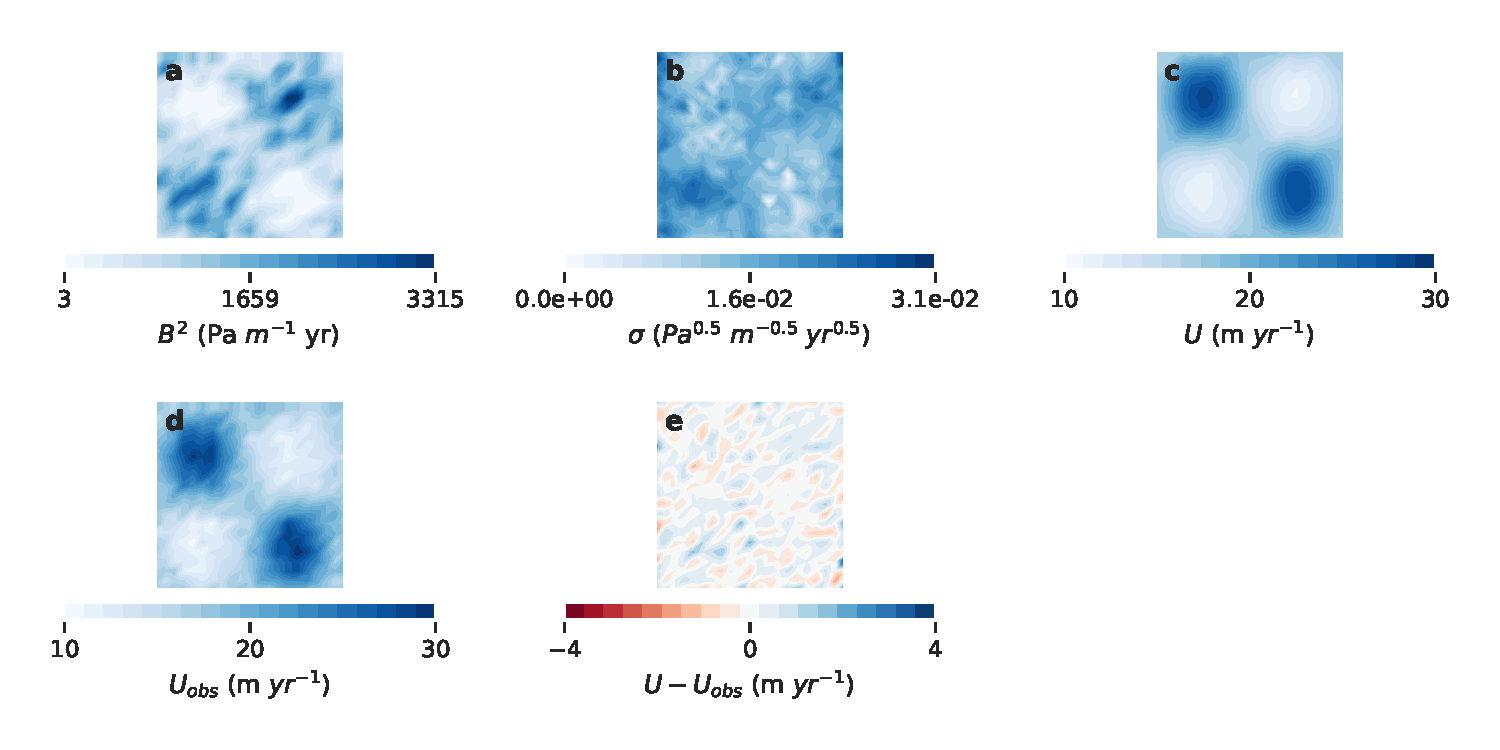
\includegraphics[width=13cm]{./figures/inv_results_rc1e4.pdf}
  \caption[IsmipC Inversion Results for Low Regularization.]{IsmipC inversion results for lower regularization. Panels as above. }
      \label{fig:inv_results_rc1e4}
\end{figure}

\subsubsection{Eigenvectors}

\begin{figure}[!htbp]
  \centering
  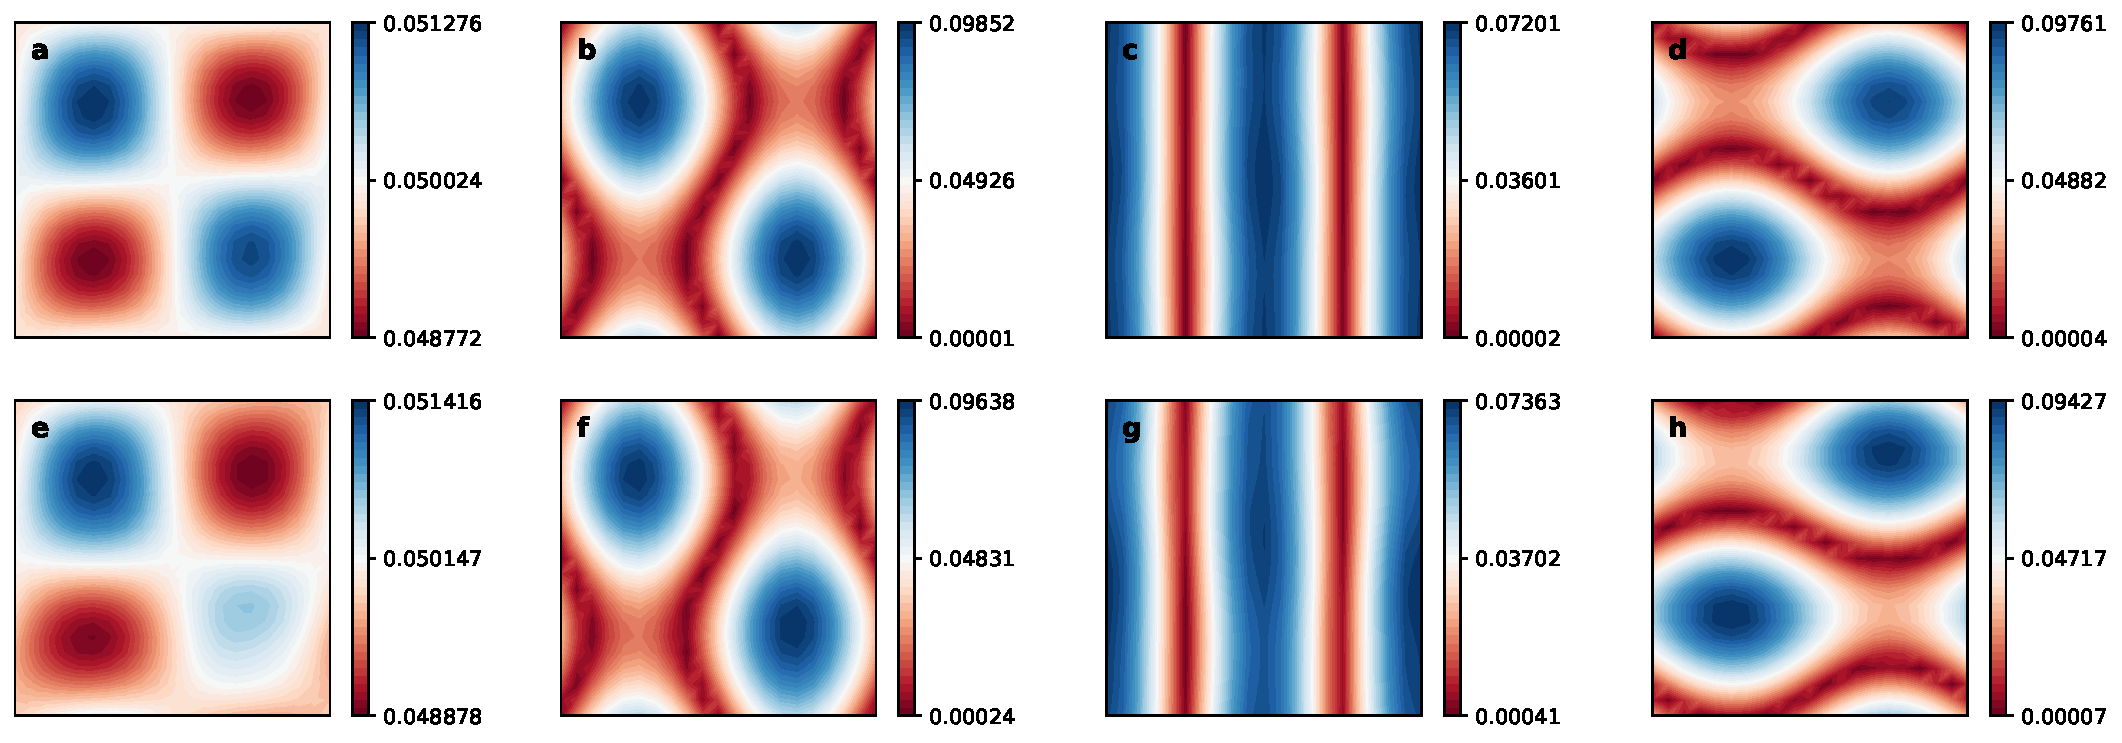
\includegraphics[width=13cm]{./figures/leading_eigenvectors_0.pdf}
  \caption[IsmipC Basal Drag Leading Eigenvectors.]{Leading four constrained modes of the inverted basal drag.}
      \label{fig:leading_eigenvectors_0}
\end{figure}


Which modes of the basal drag are well constrained by the data? These are described the eigendecomposition we performed earlier. Let's plot them for experiments {\tt uq\_rc\_1e6} and {\tt uq\_rc\_1e4}. The command required is:

\begin{spverbatim}
>python plot_leading_eigenfuncs.py
\end{spverbatim}

At the top of the file you can specify the simulation folders and the output location. The default output folder is {\tt output/ismipC/plots}. Four eigenvectors are plotted by default, with the parameter {\tt e\_offset} specifying the first eigenvector to plot. The order of the eigenvectors corresponds to how well constrained they are. 

Two figures are shown. In each figure, the top row corresponds to simulation {\tt uq\_rc\_1e6}, and the bottom panel to simulation {\tt uq\_rc\_1e4}. The first four eigenvectors are shown in Figure \ref{fig:leading_eigenvectors_0}, while eigenvectors 30-33 are shown in Figure \ref{fig:leading_eigenvectors_30}. Set the parameter {\tt e\_offset} to 30 to reproduce the second plot.  Observe that the top constrained modes between simulations are nearly identical. Also notice that well constrained modes correspond to lower frequencies.

\begin{figure}[!htbp]
  \centering
  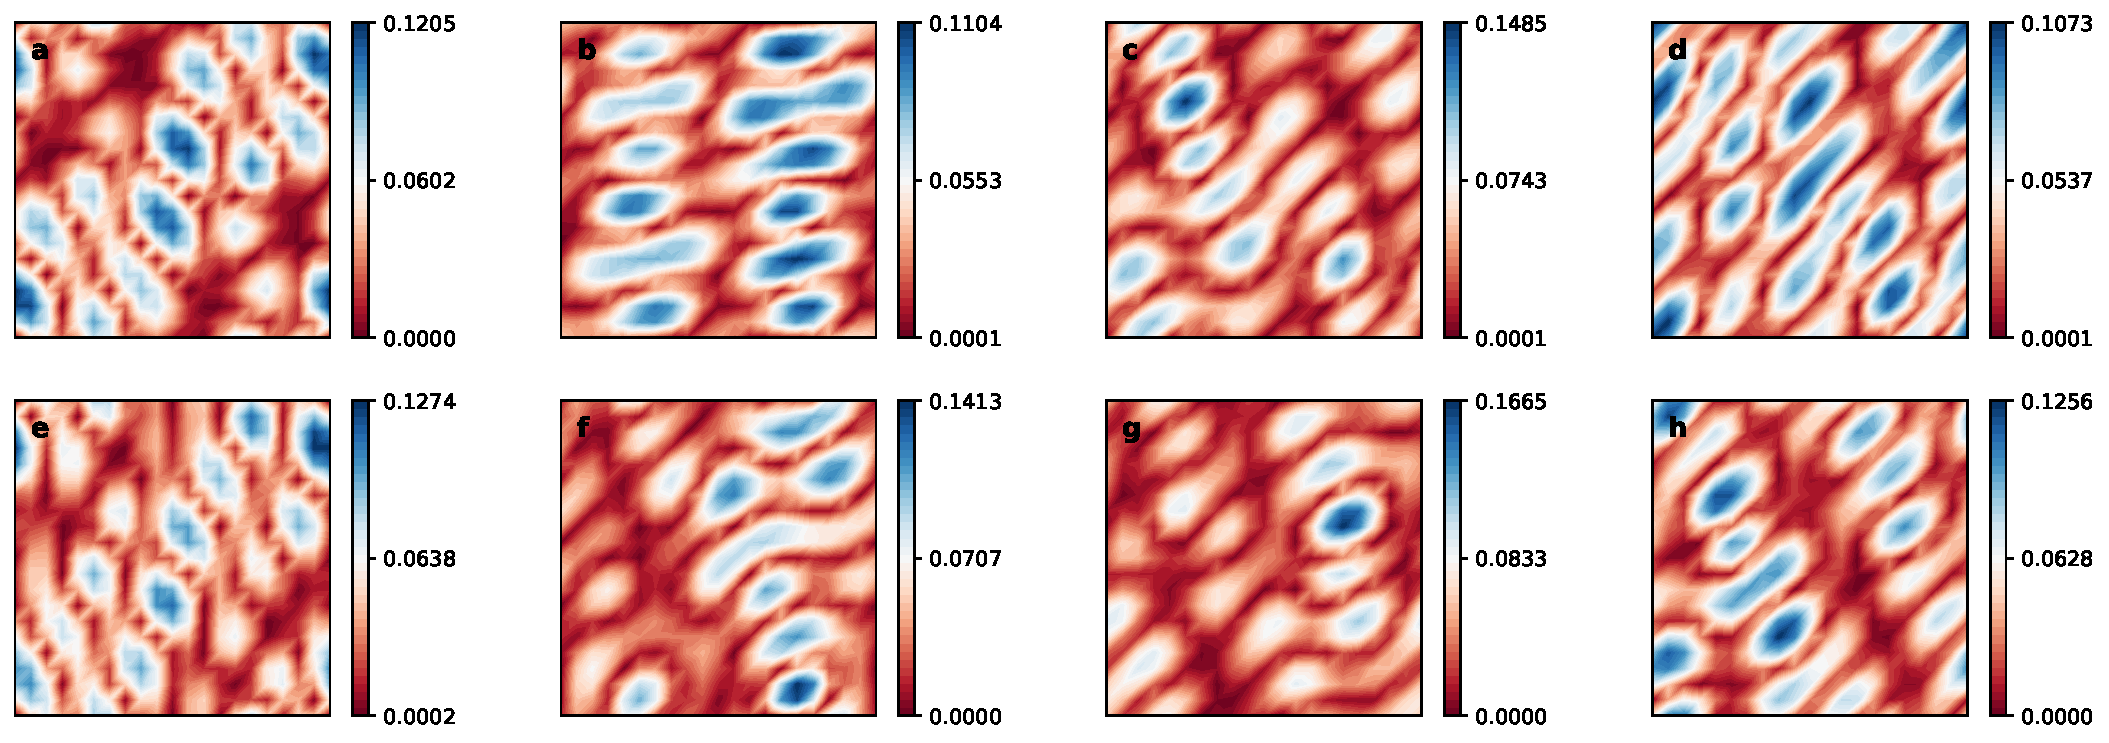
\includegraphics[width=13cm]{./figures/leading_eigenvectors_30.pdf}
  \caption[IsmipC Basal Drag Eigenvectors 30-33.]{Eigenvectors 30-33, showing less well constrained modes of basal drag. }
      \label{fig:leading_eigenvectors_30}
\end{figure}

\subsubsection{Eigenvalues}

How well constrained are the eigenvectors we plotted previously? This information is given by the corresponding eigenvalues (Figure \ref{fig:grid_convergence}). We'll plot the eigenvalues for the simulations: {\tt uq\_rc\_1e6}, {\tt uq\_30x30}, and {\tt uq\_40x40} -- which differ only in their resolution. The command is:

\begin{spverbatim}
>python plot_eigenvalue_decay.py
\end{spverbatim}

Observe how the eigenvalues quickly drop-off in their magnitude, and overlay in each other. This reflects the fact that we expect the same low frequencies modes to be well constrained across different grid resolutions.

\begin{figure}[!htbp]
  \centering
  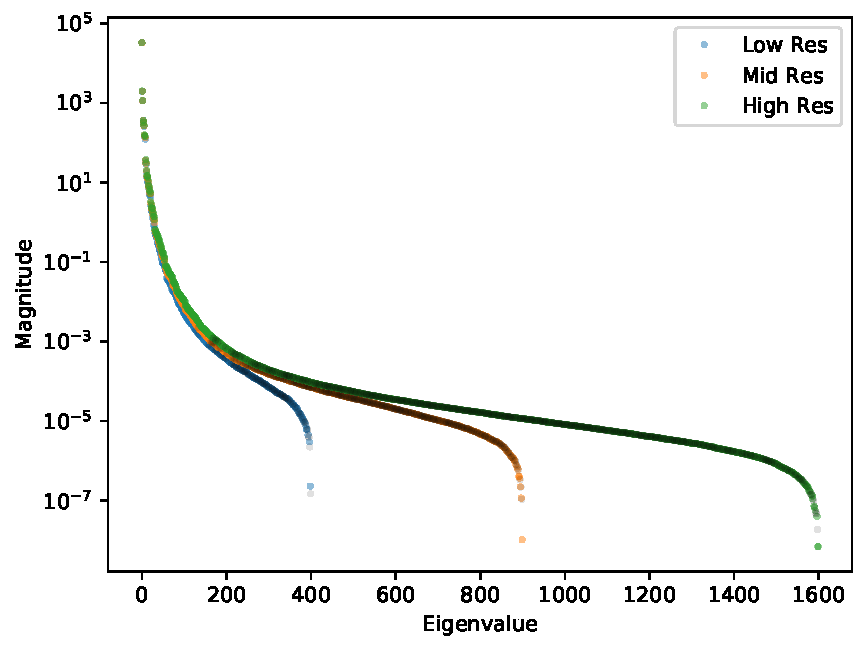
\includegraphics[width=10cm]{./figures/grid_convergence.pdf}
  \caption[Grid Convergence of Eigenvalues]{Eigenvalues of different modes of basal drag for IsmipC at low (20x20), medium (30x30), and high resolutions (40x40). Black eigenvalues correspond to negative values; they begin to appear at eigenvalues several orders of magnitude below the leading eigenvalues.  Leading eigenvalues at different resoultions closely overlay each other. }
      \label{fig:grid_convergence}
\end{figure}

\subsubsection{Quantity of Interest Probability Distribution through time}

The quantity of interest for IsmipC was defined as the integral of ice thickness squared over the domain. Using uncertainty quantification techniques, FenicsIce determines not only a point estimate of the quantity of interest through time, but also a standard deviation (based on an assumption that it is distributed normally). Let's compare the results for simulations {\tt uq\_rc\_1e4} and {\tt uq\_rc\_1e6}:

\begin{spverbatim}
>python plot_paths.py
\end{spverbatim}

\begin{figure}[!htbp]
  \centering
  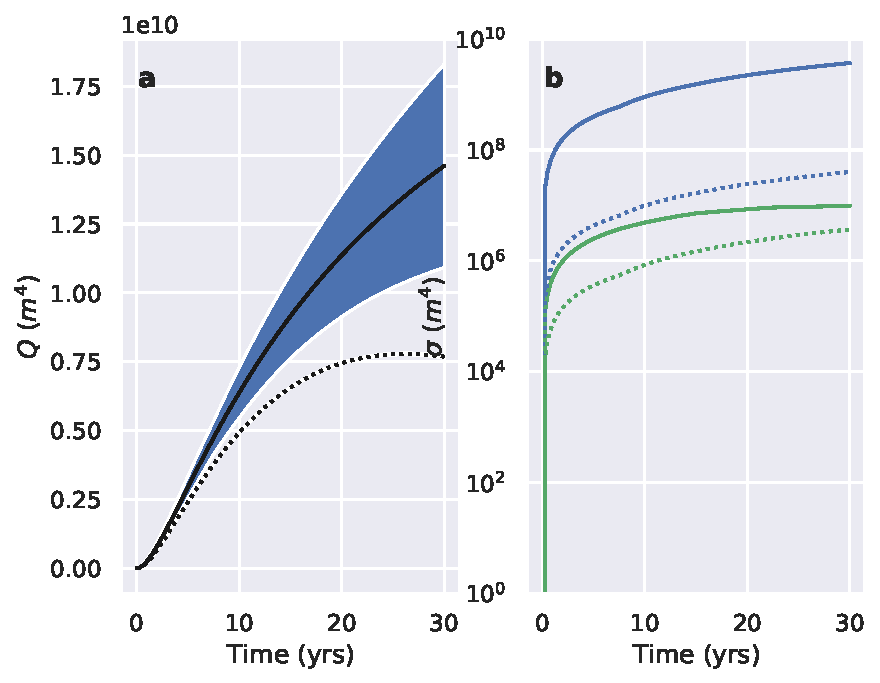
\includegraphics[width=10cm]{./figures/run_paths.pdf}
  \caption[Quantity of Interest through Time]{Probability distribution of the quantity of interest through time. The quantity of interest for IsmipC is the integral of height squared over the domain. \textbf{(a)} quantity of interest and a 2-sigma envelope.  Dashed line shows simulation {\tt uq\_rc\_1e6} and the solid line shows simulation {\tt uq\_rc\_1e4}.  The blue prior only envelope for {\tt uq\_rc\_1e4} is the only one visible. \textbf{(b)} 2-sigma values for the quantity of interest through time. Solid line corresponds to {\tt uq\_rc\_1e4} while dashed line indicates {\tt uq\_rc\_1e6}. Blue lines correspond to the prior-only standard deviation, while the dashed line shows the standard deviation after data assimilation.}
      \label{fig:run_paths}
\end{figure}

The plots show the 2-sigma envelope if we consider only the prior (regularization), as well as the prior plus information from the data. While the prior-only envelope for simulation {\tt uq\_rc\_1e4} shows large uncertainty on the order of the quantity of interest, increasing the regularization by two orders of magnitude ({\tt uq\_rc\_1e4}) collapses the uncertainty by 2-3 orders. When data is taken into consideration, it is clear that the basal drag modes relevant to the quantity of interest are well constrained.

\subsubsection{Quantity of Interest with respect to alpha}

FenicsIce can calculate how the quantity of interest at a given point in time depends on basal drag (parameterized by alpha) ($\frac{d QOI_{t}}{d \alpha}$). With this we can understand which parts of the basal drag field are the most important in determing the quantity of interest. To make this plot using the final timestep, run the following:

\begin{spverbatim}
>python plot_dq_ts.py
\end{spverbatim}

\begin{figure}[!htbp]
  \centering
  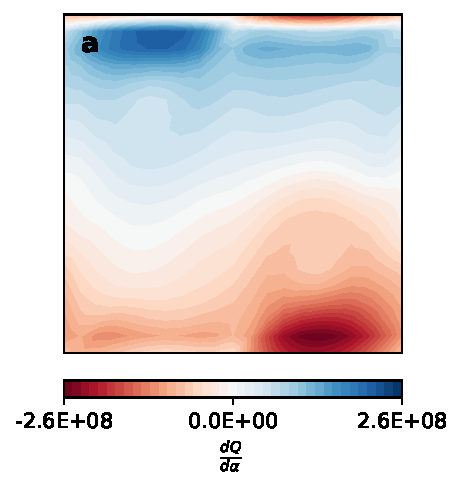
\includegraphics[width=10cm]{./figures/dq_ts.pdf}
  \caption[Derivative of Quantity of Interest at last timestep w.r.t to alpha]{The derivative of the quantity of interest at the last timestep with respect to alpha. }
      \label{fig:grid_convergence}
\end{figure}





\section{IsmipC}\label{IsmipC}

\begin{table}[!htpb] 
\centering
\begin{tabular}{llll}
\hline
 Symbol & Constant  & Value  & Units   \\
 \hline
 A &  Ice-flow parameter &  $10^{-16}$ &  \si{\pascal\tothe{n}\per\year}  \\
 $\rho_i$ & Ice Density &  910 &   \si{\kilo\gram\per\metre\cubed}   \\
  g & Gravitational constant  & 9.81  & \si{\metre\per\second\squared}   \\
  n & Exponent in Glen's Flow law  & 3  &   \\
  $t_y$ & Seconds per year  & 31556926  & \si{\second\per\year}   \\
 \hline
\end{tabular}
\caption[Constants for ISMIP-HOM experiments.]{Constants for ISMIP-HOM experiments}
    \label{table:ISMIPparam}
\end{table}


Ice Sheet Model Intercomparison Project for Higher-Order ice sheet Models (ISMIP-HOM) is a set of standardized simulations used in the glaciology community for model intercomparison. Due to its familiarity, and simple setup, Experiment C was selected for the tutorial in this user-guide. It allows many aspects of uncertainty quantification to be explored in a simple domain.

The domain of Experiment C is a square domain with periodic boundary conditions on all four boundaries. The surface and basal topography are prescribed as:

%
\begin{equation}
s(x,y) = -x \cdot tan(0.1\si{\degree})
\label{eq:ismipCS}
\end{equation} 
%
\begin{equation}
b(x,y) = s(x,y) - 1000
\label{eq:ismipCB}
\end{equation} 
%


In Experiment C, basal drag is parameterized with a linear sliding law, with the drag coefficient prescribed as:
%
\begin{equation}
\beta = [1000 + 1000sin(\omega x)cos(\omega y)] \cdot t_y^{-1}
\label{eq:ismipCBD}
\end{equation} 
%
where $t_y$ is the number of seconds in a year, converting $\beta$ to SI units.

\section{Tutorial 2 : A Walkthrough of Smith Glacier} \label{sec:smith}

This section walks through a fenics\_ice simulation of the Smith Glacier domain (actually Smith, Pope and Kohler Glaciers), from mesh generation, definition of .toml file, through to analysis of results.

\subsection{Mesh Generation}

Finite element simulations start with a mesh.
The `Smith' mesh (Fig. \ref{fig:smithmesh}) is an unstructured grid with highly variable resolution (edge length).
This mesh was generated using the script {\tt smith\_mesh\_metric\_mmg.py} in {\tt fice\_toolbox/meshing}.
This section will describe the mesh generation process with reference to that script.
The script depends on the following libraries which can (I think) be installed with conda:
\begin{itemize}
\item netCDF4
\item gmsh
\item meshio
\end{itemize}

and the local library `meshtools' which exists in the same directory as smith\_mesh\_metric\_mmg.py.
It also requires a local MMG installation. See {\tt fice\_toolbox/meshing/README.md} for details of an installation script for MMG v5.5.2.

We start with two datasets:

\href{https://nsidc.org/data/nsidc-0545}{ASE velocity} from which we can compute strain rates.

\href{https://nsidc.org/data/NSIDC-0756/versions/1}{BedMachine} which provides several geometry fields and, importantly, a raster mask defining ice, ocean, nunatak, etc.

Note that the script refers to a `mask\_h5' dataset, but this is just an alternative to using the BedMachine mask.

Velocity data are loaded and eigenstrains are computed. \textbf{Eigen}strain is important for an isotropic mesh because it is invariant under rotation. The mean eigenstrain for each cell through the timeseries is computed, and this also helps to fill holes in the data.

The actual mesh generation occurs in two phases:
\begin{enumerate}
\item Initial uniform-resolution mesh generated by Gmsh.
\item Mesh refinement using strain metric in MMG.
\end{enumerate}

The purpose of the first phase is to define points at which the metric can be interpolated. This interpolated metric then defines the final target edge length as a field.

This script also automatically generates appropriate boundary labels for ice/ocean (calving) and ice/ice (edge of domain) boundaries by analysing the BedMachine mask. It writes out the required `\_ff.xdmf' and `\_ff.h5' files containing this boundary info in FEniCS-ready format. It also spits out a `\_BCs.txt' file which lists each boundary label and its associated boundary type (ocean, ice). This file helps the user write the [[BC]] sections in the .toml file.

To conclude, given the following specification in {\tt smith\_mesh\_metric\_mmg.py}:

\begin{spverbatim}
mesh_outfile = ``smith_variable_ocean''
\end{spverbatim}

the script should produce the following output files:

\begin{itemize}
\item smith\_variable\_ocean.xdmf -- FEniCS XDMF mesh format
\item smith\_variable\_ocean.h5 -- HDF5 data file for above
\item smith\_variable\_ocean\_ff.xdmf -- FEniCS 'MeshValueCollection' containing FacetFunction
\item smith\_variable\_ocean\_ff.h5 -- HDF5 data file for above
\item smith\_variable\_ocean\_BCs.txt -- Human readable description of BC labels
\end{itemize}

\subsection{Input Data}

In addition to the 2D mesh, we need data describing the ice thickness, bed elevation, SMB, melt rates, etc. This is accomplished by the script\\
 {\tt fice\_toolbox/cases/Smith/BedMachine\_data/scripts/bedsurf\_smith\_bedmachine.py}.

This script loads bedrock bedrock elevation, ice thickness \& ice surface elevation from BedMachine for a specified region. It also applies a gaussian filter to the surface elevation; this is necessary because the surface elevation is sufficiently high resolution to pick up crevasses. These crevasses are then transmitted to the ice-base elevation unless filtering is applied. The strength of gaussian filtering is controlled by the -sigma argument. The script produces an HDF5 data file called `smith\_bedmachine.h5' which, along with the 2D mesh, completely defines the geometry.

The background field for beta is derived from temperature estimates from Frank Pattyn's work. Dan should know about this. It's processed by the script\\
 {\tt fice\_toolbox/cases/Smith/BedMachine\_data/scripts/pattyn\_temp.py}. Note that the approach to initializing alpha and beta differs. An initial guess for alpha is derived internally by fenics\_ice in {\tt model.gen\_alpha}. However, for beta, the initial guess is derived from temperature data, and furthermore, the inversion \emph{penalises divergence from this initial guess}. This is not the case with alpha.

So far, I have not addressed the need for \emph{basal melt and surface mass balance}. For now, SMB for the Smith domain is set to a constant 0.38 m/a and no basal melting is imposed. The files which describe these fields were generated using\\ {\tt fenics\_ice/input/smith\_500m\_input/gen\_smith\_domain.py}; this is Conrad's stuff.

\subsection{Running Simulations}

From within my `fenics\_ice' conda environment, I use a script containing the following code to run all phases of a simulation on 12 cores on the machine called `bow':

\begin{spverbatim}
#contents of run.sh
mpirun -n 12 python ~/sources/fenics_ice/runs/run_eigendec.py smith.toml
mpirun -n 12 python ~/sources/fenics_ice/runs/run_forward.py smith.toml
mpirun -n 12 python ~/sources/fenics_ice/runs/run_invsigma.py smith.toml
mpirun -n 12 python ~/sources/fenics_ice/runs/run_errorprop.py smith.toml
\end{spverbatim}

I call the script like this:
\begin{spverbatim}
nohup bash run.sh | tee log_smith_demo_run & disown
\end{spverbatim}

The combination of `nohup' and `\& disown' allows the simulation to run in the background once I end the ssh connection. This is \textbf{strongly} recommended, because if the connection drops accidentally the simulation will halt and there's no restart facility. Piping the output to `tee' creates a log file. Alternatively, if you wanted to keep separate logs for each run phase, you could add a {\tt | tee} on the end of each command in {\tt run.sh}.

In the next couple of sections I'll describe some parts of the inversion \& eigendecomposition process. This is only 2 of the 5 run phases, but there's not much to say about the rest. They are described elsewhere in this document.

\subsection{Inversion \& L-curves}

The inverse model uses L-BFGS to minimize the cost function. Parameters for L-BFGS include, but are not limited to:

\begin{spverbatim}
[inversion]
max_iter = 500       # Upper limit on L-BFGS iterations
ftol = 1e-8          # Stopping criterion: decrease in J
gtol = 1e-12         # Stopping criterion: decrease in dJ
delta_lbfgs = 1.0e3  # initial theta scaling (off by default)
\end{spverbatim}

The following parameters describe the regularisation terms, and were obtained via L-curve analysis (e.g. Fig. \ref{fig:smith_lcurve}):
\begin{spverbatim}
gamma_alpha = 1e2
delta_alpha = 1e-5
gamma_beta = 1.0e2
delta_beta = 1e-5
delta_beta_gnd = 3e-5
\end{spverbatim}


L-curve analysis plots, for a range of parameter values, the cost function mismatch term (x-axis) against the regularisation term (y-axis).
In general, the goal is to pick the largest regularisation term which does not increase the mismatch term.
This can be quite subjective, and for the purposes of uncertainty quantification, it is common to slightly \emph{over}regularise.

I wrote a couple of scripts in {\tt fice\_toolbox} to help perform the parameter sweeps required for an L-curve analysis, and to plot the results. The script {\tt param\_sweep.py} (Section \ref{sec:scripts}) generates a series of .toml files and a shell script to run each in turn. The script {\tt smith\_l\_curve\_rough.py} plots the L-curve.

\begin{figure}[!htbp]
  \centering
  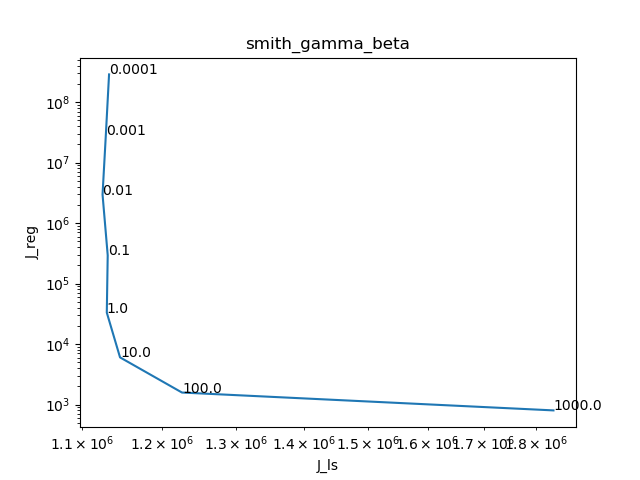
\includegraphics[width=10cm]{./figures/smith_gamma_beta.png}
  \caption[L-curve for delta\_beta for Smith Glacier]{L-curve for delta\_beta for Smith Glacier. Produced using script `smith\_l\_curve\_rough.py'}
      \label{fig:smith_lcurve}
\end{figure}


\subsection{Eigendecomposition}

I tend to set {\tt num\_eig} in the {\tt [eigendec]} .toml section to a large number (15000) and then just set it running (This could be improved -  see \ref{sec:improveed}).
fenics\_ice writes out both the eigenfunctions and eigenvalues progressively, so you can monitor the latest results as the simulation progresses.
Based on advice from James, I leave the eigendecomposition running until the smallest absolute eigenvalue reaches 1/3.
This can be checked by inspecting the file {\tt output/run\_name\_eigvals.p}.
There should be a script called {\tt eigvals.py} in with the Smith run files which prints out the smallest eigenvalue and also plots the eigenspectrum.

Note that the use of {\tt nohup} means that, to halt the ED while it's running requires killing the running job. I achieve this via:

\begin{spverbatim}
  pkill -9 python
\end{spverbatim}

This is only really safe because I know the only python job that I have \emph{permission} to kill is the running fenics\_ice simulation. This wouldn't work properly if, for example, you were running multiple simulations at the same time. In this case, it might be worth investigating {\tt screen} or {\tt tmux} for finer grained control of running simulations.
Alternatively, run on a system with a proper job queuing system like Torque or Slurm.

\subsection{Results in Paraview}

Once the simulation completes, results can be downloaded from the {\tt output} directory using rsync, then viewed in Paraview. Output formats and how these can be loaded into Paraview are described in Section \ref{sec:output}. Figure \ref{fig:smith_ed} shows the alpha component of the 21st eigenfunction for the Smith simulation. Note that I've changed the colour scheme and range to improve the visualisation, and that the `time' is set to 20 of 12355. Paraview interprets the series of eigenfunctions as a timeseries.

\begin{figure}[!htbp]
  \centering
  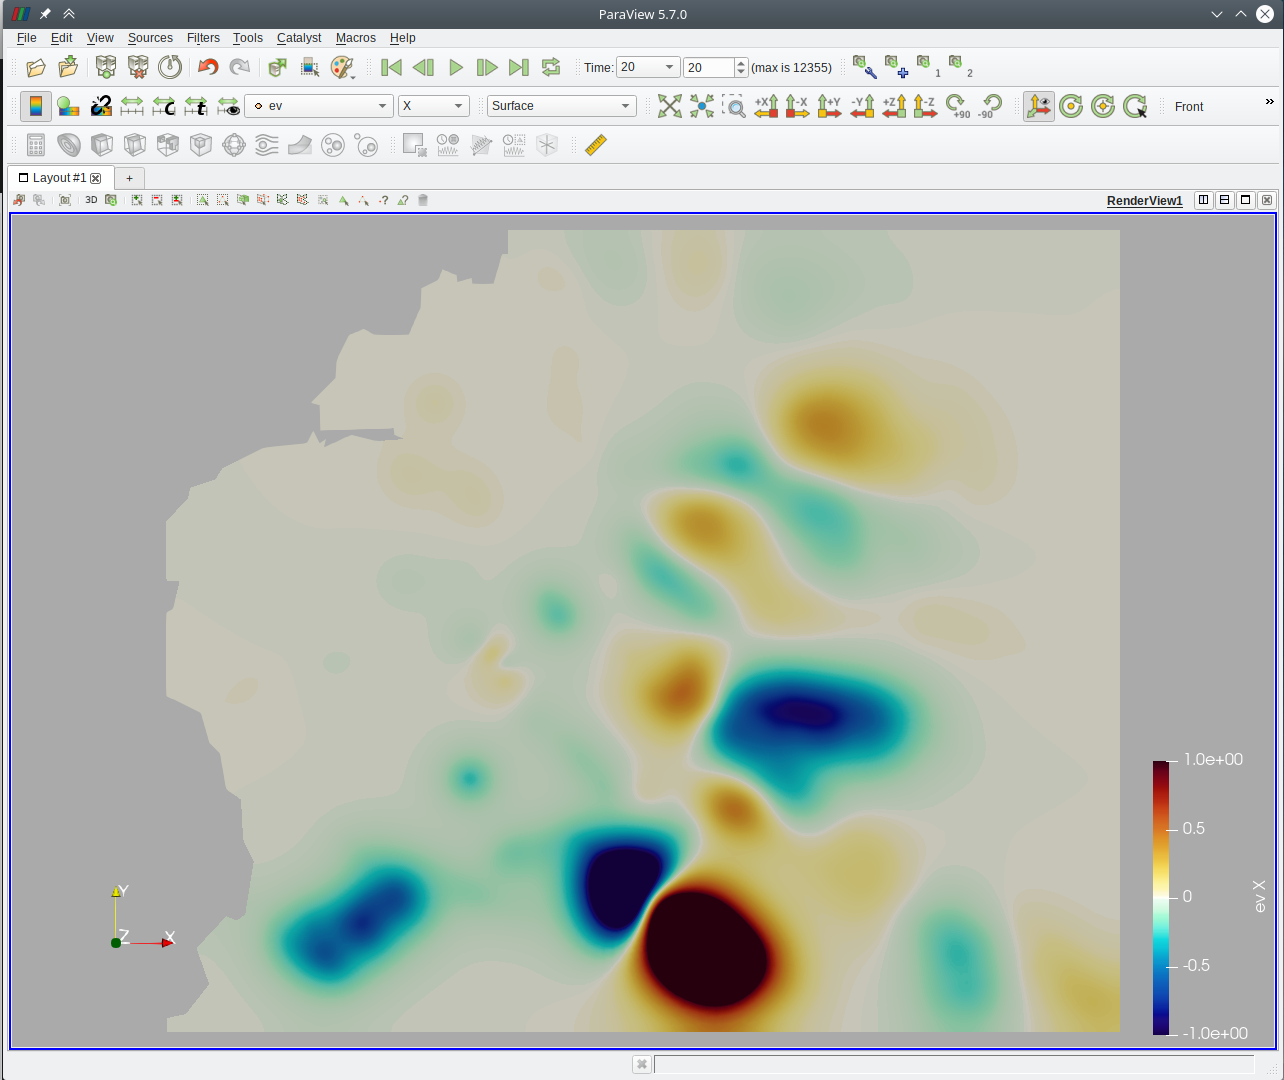
\includegraphics[width=14cm]{./figures/smith_21_ev_alpha.png}
  \caption[]{Alpha component of 21st eigenfunction of the Smith simulation.}
      \label{fig:smith_ed}
\end{figure}

\section{Development Priorities}

Here's some thoughts on things which ought be improved or fixed, which I didn't quite get round to.

\subsection{Run phases \& restarts}

At the moment, there's no way to specify that a `run\_name' should restart from a different `run\_name'. For example, something I've wanted to do a couple of times is to run the same simulation twice, once where I eigendecompose only the alpha control function (e.g. `Smith\_aonly'), and once where I do a dual eigendecomposition (`Smith\_dual'). For \textbf{both} of these simulations, I might want to \emph{invert} for both alpha \& beta, so both simulations have the same initial inversion phase, which we might call `Smith\_invertdual'. But at the moment, fenics\_ice can't be instructed to run the eigendecomposition phase `Smith\_aonly' from the inversion phase `Smith\_invertdual'. If you were short on computing resources, the way to achieve this would be to create symlinks for each of the result files (`Smith\_aonly\_alpha.pvd' \textrightarrow  `Smith\_invertdual\_alpha.pvd'), but in practice I usually just end up running the same inversion phase twice, which is very inefficient. The elegant solution to this would be to allow the user to specify different 'run\_phase\_names' instead of a single 'run\_name'.

\subsection{Output Formats}

There's no way at the moment to write multiple variables to a single PVD/PVTU file. This is a feature that you won't miss because you've never had it, but it's \textbf{so useful} because it means Paraview is naturally aware of multiple variables defined on the same domain. This means you can perform all sorts of calculations on combinations of variables. It would also significantly reduce clutter (fewer files). Elmer does this and it should be achievable.

\subsection{Sliding Laws}

At present only a linear or a Budd-style sliding law is available. Dan and I discussed adding a Schoof law. This would be good because, as we've discussed, it might be less susceptible to issues of differentiability at the grounding line. It's also quite a popular sliding law, and it may be that future publications with fenics\_ice are criticised for not investigating this law.

\subsection{Eigendecomposition} \label{sec:improveed}

An easy \& quite useful improvement to the eigendecomposition would be to have it halt once the smallest eigenvalue reaches 1/3, which James advises is the critical point beyond which we really don't care about the rest of the eigenspectrum. This would be a pretty straight forward addition to the slepc monitor callback.

\subsection{Time Dependent Inversions}

This is the big one - we'd like to be able to feed in velocity observations from multiple points in time to better constrain basal/rheological conditions. As an intermediate step, Dan's idea was to feed in a single snapshot accompanied by a thickening/thinning trend (dH/dt).

\subsection{Code structure \& OO Best Practices}

At the moment, I'm not totally happy with the structure of fenics\_ice in terms of the relationship between the model \& solver objects. It works fine, but it may hobble future development slightly. The solver class is a bit bloated and it's responsible for too many things. Why is a single 'solver' object responsible for both the SSA equations \& thickness advection? If temperature evolution was added, do we want a separate solver for that?

\subsection{Expanding Test Coverage}

The integration tests in test\_runs.py provide good overall coverage of every phase of a simulation. However, the unit tests in test\_model.py don't cover most of the code. Maybe this is OK - if the integration tests produce the right results, then you can be fairly confident you've not broken anything. But when things do go wrong, better coverage in the unit tests might make debugging easier.

\subsection{Repo bloat}

The fenics\_ice is way bigger than it needs to be because there's some massive datafiles which were accidentally committed way back when. Although these were subsequently deleted, they were never purged from history, meaning they still exist in the repo history. Purging these would make the repo a lot smaller, and probably isn't particularly hard to do.

\section{Publications}
This section will be updated as publications with Fenics Ice appear.

\section{Citing}
This section will be updated when the GMD paper is published.



\newpage
\bibliography{references}
\bibliographystyle{plain}



\end{document} 